%
% Lecture notes for the Software and Systems Verification (VIMIMA01) course
%

%TODO or 12pt? or use a5paper? or use ebook?
\documentclass[10pt,a4paper,oneside]{memoir}

%%%%%%%%%%%%%%%%%%%%%%%%%%%%%%%%%%%%%%%%%%%%%%%%%
% Package imports
%%%%%%%%%%%%%%%%%%%%%%%%%%%%%%%%%%%%%%%%%%%%%%%%%

%TODO find a decent font
\usepackage[T1]{fontenc}		% use T1 encoding instead of the classic OT1
\usepackage[utf8]{inputenc}		% The package translates various standard and other input encodings into a ‘LaTeX internal language’
\usepackage{graphicx}			% Enhanced support for graphics

%TODO use other style that uses annotations? Or put comments into note/addendum?
%TODO separate must have and extra references?
\usepackage[backend=biber,style=alphabetic,bibencoding=utf8,giveninits=true]{biblatex}
\usepackage[unicode,pdftex]{hyperref}	% Extensive support for hypertext links in LaTeX



%%%%%%%%%%%%%%%%%%%%%%%%%%%%%%%%%%%%%%%%%%%%%%%%%
% Settings
%%%%%%%%%%%%%%%%%%%%%%%%%%%%%%%%%%%%%%%%%%%%%%%%%

\addbibresource{bib/references.bib}

\hypersetup{
pdfauthor = {Zoltan Micskei (ed.)},
pdftitle = {Software and Systems Verification},
pdfsubject = {VIMIMA01 course at BME},
pdfkeywords = {testing, requirements, static analysis}, 
pdfcreator = {LaTeX},
pdfproducer = {pdflatex},
bookmarksnumbered=true,
}

\firmlists				% reduces the space between list items, see \defaultlists and \tightlists

\midsloppy				% TeX tries very hard to keep text lines justified, this relaxes it a bit (but not as much ah \sloppy)


%%%%%%%%%%%%%%%%%%%%%%%%%%%%%%%%%%%%%%%%%%%%%%%%%
% New commands and environments
%%%%%%%%%%%%%%%%%%%%%%%%%%%%%%%%%%%%%%%%%%%%%%%%%


%%%%%%%%%%%%%%%%%%%%%%%%%%%%%%%%%%%%%%%%%%%%%%%%%
% Main document
%%%%%%%%%%%%%%%%%%%%%%%%%%%%%%%%%%%%%%%%%%%%%%%%%

\begin{document}

%
% Front matter: title pages, acknowledgement, summary, TOC
% (See memdesign.pdf on the usual parts and order)
%
\frontmatter

%%%%%%%%%%%%%%%%%%%%%%%%%%%%%%%%%%%%%%%%%%%%%%%%%%%%%%%%%%%%%%%%
% Title and copyright page
%%%%%%%%%%%%%%%%%%%%%%%%%%%%%%%%%%%%%%%%%%%%%%%%%%%%%%%%%%%%%%%%

% do not print page numbers on title and copyright page
\pagestyle{empty}

%TODO customize title page
\title{Software and Systems Verification}
\author{Zoltan Micskei (ed.)}

\maketitle 

\clearpage

%
% Copyright page
%
\vspace*{0.1\textheight}

{\setlength{\parindent}{0cm}
Zoltán Micskei (ed.) \\

Based on the work of Istvan Majzik, Daniel Darvas, Akos Hajdu, David Honfi \\

\url{http://inf.mit.bme.hu/en/edu/courses/swsv} \\
    
September 2016 \\
    
Budapesti Műszaki és Gazdaságtudományi Egyetem (BME) \\
Villamosmérnöki és Informatikai Kar (VIK) \\
Méréstechnika és Információs Rendszerek Tanszék (MIT) \\
    
Budapest University of Technology and Economics \\
Faculty of Electrical Engineering and Informatics \\
Department of Measurement and Information Systems \\
    
H-1117 Budapest, Magyar tudósok körútja 2.

\clearpage

%
% From now on, print page numbers and titles in the header
% See Section 7.2 in memman.pdf for possible pagestyles
%
\pagestyle{headings}


%%%%%%%%%%%%%%%%%%%%%%%%%%%%%%%%%%%%%%%%%%%%%%%%%%%%%%%%%%%%%%%%
% Preface
%%%%%%%%%%%%%%%%%%%%%%%%%%%%%%%%%%%%%%%%%%%%%%%%%%%%%%%%%%%%%%%%

\section*{Preface}

Lecture notes for the Master level course at Budapest University of Technology and Economics

Goal of the course

Main topics

Learning Objectives, knowledge levels...

Hungarian terms \cite{htb-glossary}

\tableofcontents

%
% Main content
%
\mainmatter

\part{Overview}

\chapter{Introduction}
\label{cha:introduction}

Software systems \cite{ieee-24765}

Verification and validation

Overview of techniques
\chapter{Critical Systems}


\begin{figure}[ht]
    \centering
    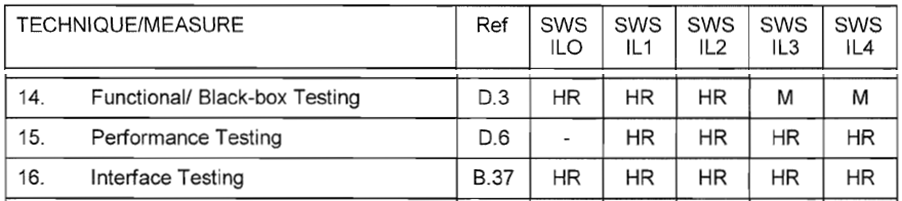
\includegraphics[width=0.9\textwidth]{figures/en-50128-example-recommended-techniques}
    \caption{Example: Recommendation of techniques in EN 50128}
    \label{fig:overview:en-50128-technique-recommendation}
\end{figure}

\section{Hungarian terms}

\begin{table}
    \centering
    \small
    \caption{Hungarian terms for critical systems}
    \begin{tabular}{ll}
        \toprule
        \textbf{English} & \textbf{Hungarian} \\
        \midrule
        assessor & értékelő \\
        availability & rendelkezésre állás \\
        certification & tanúsítvány \\
        fault tolerance & hibatűrés \\
        reliability & megbízhatóság \\
        risk & kockázat \\
        safety & biztonságosság \\
        safety integrity level & biztonságintegritási szint \\
        safety-critical system & biztonságkritikus rendszer \\
        standard & szabvány \\
        tolerable hazard rate & elviselhető veszélygyakoriság \\
        \bottomrule
    \end{tabular}
    \label{tab:overview:hungarian-terms-critical-systems}
\end{table} 

\part{Static Techniques}

%TODO put some description for the part but before the first chapter?
% These techniques do not execute the system.

\chapter{Verifying specifications and requirements}
\label{cha:specifications}



\section{Hungarian terms}

\begin{table}
    \centering
    \small
    \caption{Hungarian terms for verifying specifications}
    \begin{tabular}{ll}
        \toprule
        \textbf{English} & \textbf{Hungarian} \\
        \midrule
        impact analysis & hatáselemzés \\
        inspection & inspekció \\
        peer review & egyenrangú felülvizsgálat \\
        requirement & követelmény \\
        review & felülvizsgálat \\
        scribe & jegyzőkönyv vezető \\
        specification & specifikáció \\
        traceability & nyomonkövethetőség \\
        use case & használati eset \\
        walkthrough & átvizsgálás \\
        \bottomrule
        \end{tabular}
        \label{tab:overview:hungarian-terms-specifications}
        \end{table} 
\chapter{Verifying source code}


\section{Hungarian terms}

\begin{table}[ht]
    \centering
    \small
    \caption{Hungarian terms for verifying source code chapter}
    \begin{tabular}{ll}
        \toprule
        \textbf{English} & \textbf{Hungarian} \\
        \midrule
        abstract interpretation & absztrakt interpretáció \\
        coding guideline & kódolási ajánlások \\
        false negative result & téves siker eredmény \\
        false positive result & téves hiba eredmény \\
        static analysis & statikus elemzés \\
        \bottomrule
        \end{tabular}
        \label{tab:overview:hungarian-terms-code}
        \end{table}

\part{Dynamic Techniques}

\chapter{Overview of Testing Techniques}
\label{cha:overview-of-testing}

(Summary of chapter)

Testing overviews: \cite{myers-1979}, \cite{swebok-testing}

\section{Definition of Testing}
\label{sec:definition-of-testing}

Other basic definitions

\subsubsection{Test oracle}

\begin{figure}[ht]
    \centering
    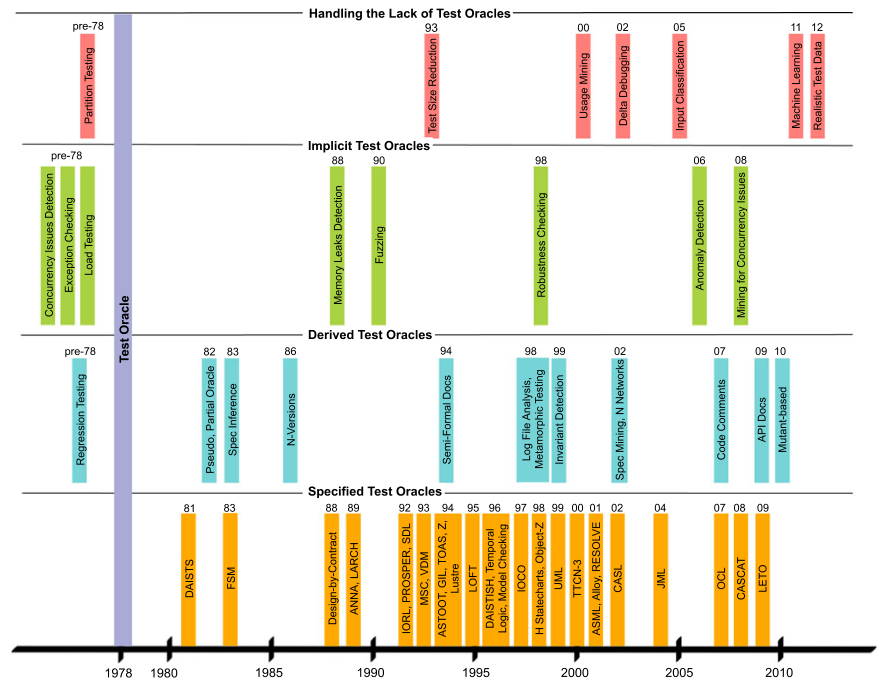
\includegraphics[width=0.9\textwidth]{figures/oracle-survey-techniques}
    \caption{Oracle techniques and concepts \cite{oracle-survey}}
    \label{fig:overview-of-testing:oracle-survey-techniques}
    \end{figure}

\section{Testing Process}
\label{sec:testing-process}

\begin{enumerate}
    \item Planning and Control
    \item Analysis and Design
    \item Implementation and Execution
    \item Evaluating Exit Criteria and Reporting    
    \item Test Closure
\end{enumerate}

Test generation will be a different chapter \cite{Anand13}.


\section{Hungarian terms}

\begin{table}[ht]
    \centering
    \small
    \caption{Hungarian terms for overview of testing chapter}
    \begin{tabular}{ll}
        \toprule
        \textbf{English} & \textbf{Hungarian} \\
        \midrule
        acceptance test & átvételi teszt \\
        exhaustive testing & kimerítő tesztelés \\
        expected outcome & elvárt eredmény \\
        exploratory testing & felderítő tesztelés \\
        fail & sikertelen teszt (bukás) \\
        oracle & orákulum \\
        pass & sikeres teszt \\
        test case & teszteset \\
        test basis & tesztbázis \\
        test design & (műszaki) teszttervezés \\
        test object & teszt tárgya \\
        test objective & tesztcél \\
        test suite & tesztkészlet \\
        \bottomrule
    \end{tabular}
    \label{tab:overview:hungarian-terms-testing-overview}
\end{table} 
\chapter{Development testing}




\section{Hungarian terms}

\begin{table}
    \centering
    \small
    \caption{Hungarian terms for developer testing}
    \begin{tabular}{ll}
        \toprule
        \textbf{English} & \textbf{Hungarian} \\
        \midrule
        driver & meghajtó \\
        isolation & izoláció / elszigetelés \\
        mock & ? \\
        stub & csonk \\
        testability & tesztelhetőség \\
        unit & egység \\
        \bottomrule
    \end{tabular}
    \label{tab:overview:hungarian-terms-developer-testing}
\end{table} 
\chapter{Specification-based test design}


\section{Hungarian terms}

\begin{table}[ht]
    \centering
    \small
    \caption{Hungarian terms for specification-based testing chapter}
    \begin{tabular}{ll}
        \toprule
        \textbf{English} & \textbf{Hungarian} \\
        \midrule
        boundary value & határérték \\
        combinatorial testing & kombinatorikus tesztelés \\
        decision table testing & döntési tábla teszt \\
        equivalence partition & ekvivalencia-partíció \\
        n-wise testing & n-szeres tesztelés \\
        pairwise testing & páronkénti tesztelés \\
        \bottomrule
    \end{tabular}
    \label{tab:overview:hungarian-terms-testing-specification}
\end{table} 
\chapter{Structure-based test design}



\section{Hungarian terms}

\begin{table}[ht]
    \centering
    \small
    \caption{Hungarian terms for structure-based testing}
    \begin{tabular}{ll}
        \toprule
        \textbf{English} & \textbf{Hungarian} \\
        \midrule
        branch & elágazás \\
        condition & feltétel \\
        control flow graph & vezérlési folyam gráf \\
        coverage & lefedettség \\        
        decision & döntés \\
        path & útvonal \\
        \bottomrule
        \end{tabular}
        \label{tab:overview:hungarian-terms-testing-structure}
        \end{table} 
\chapter{Test process and levels}



\section{Hungarian terms}

\begin{table}
    \centering
    \small
    \caption{Hungarian terms for overview}
    \begin{tabular}{ll}
        \toprule
        \textbf{English} & \textbf{Hungarian} \\
        \midrule
        exit criteria & kilépési feltétel \\
        maintainability & karbantarthatóság \\
        performance & teljesítmény \\
        integration test & integrációs teszt \\
        system test & rendszerteszt \\
        \bottomrule
        \end{tabular}
        \label{tab:overview:hungarian-terms-test-process}
\end{table} 
\chapter{Test automation}



\section{Hungarian terms}

\begin{table}[ht]
    \centering
    \small
    \caption{Hungarian terms for test automation chapter}
    \begin{tabular}{ll}
        \toprule
        \textbf{English} & \textbf{Hungarian} \\
        \midrule
        regression testing & regressziós tesztelés \\
        \bottomrule
        \end{tabular}
        \label{tab:overview:hungarian-terms-test-automation}
\end{table} 

%
% Appendices
%
\appendix
\input{content/appendix}

%
% Backmatter (unnumbered sections)
%
\backmatter

\printbibliography[heading=subbibintoc]

\end{document}

